\documentclass{dcbl/challenge}

\setdoctitle{Managing Memory and Scope}
\setdocauthor{Stephan Bökelmann}
\setdocemail{sboekelmann@ep1.rub.de}
\setdocinstitute{AG Physik der Hadronen und Kerne}
\usepackage{listings}
\usepackage{graphicx}

\begin{document}
\begin{figure}
    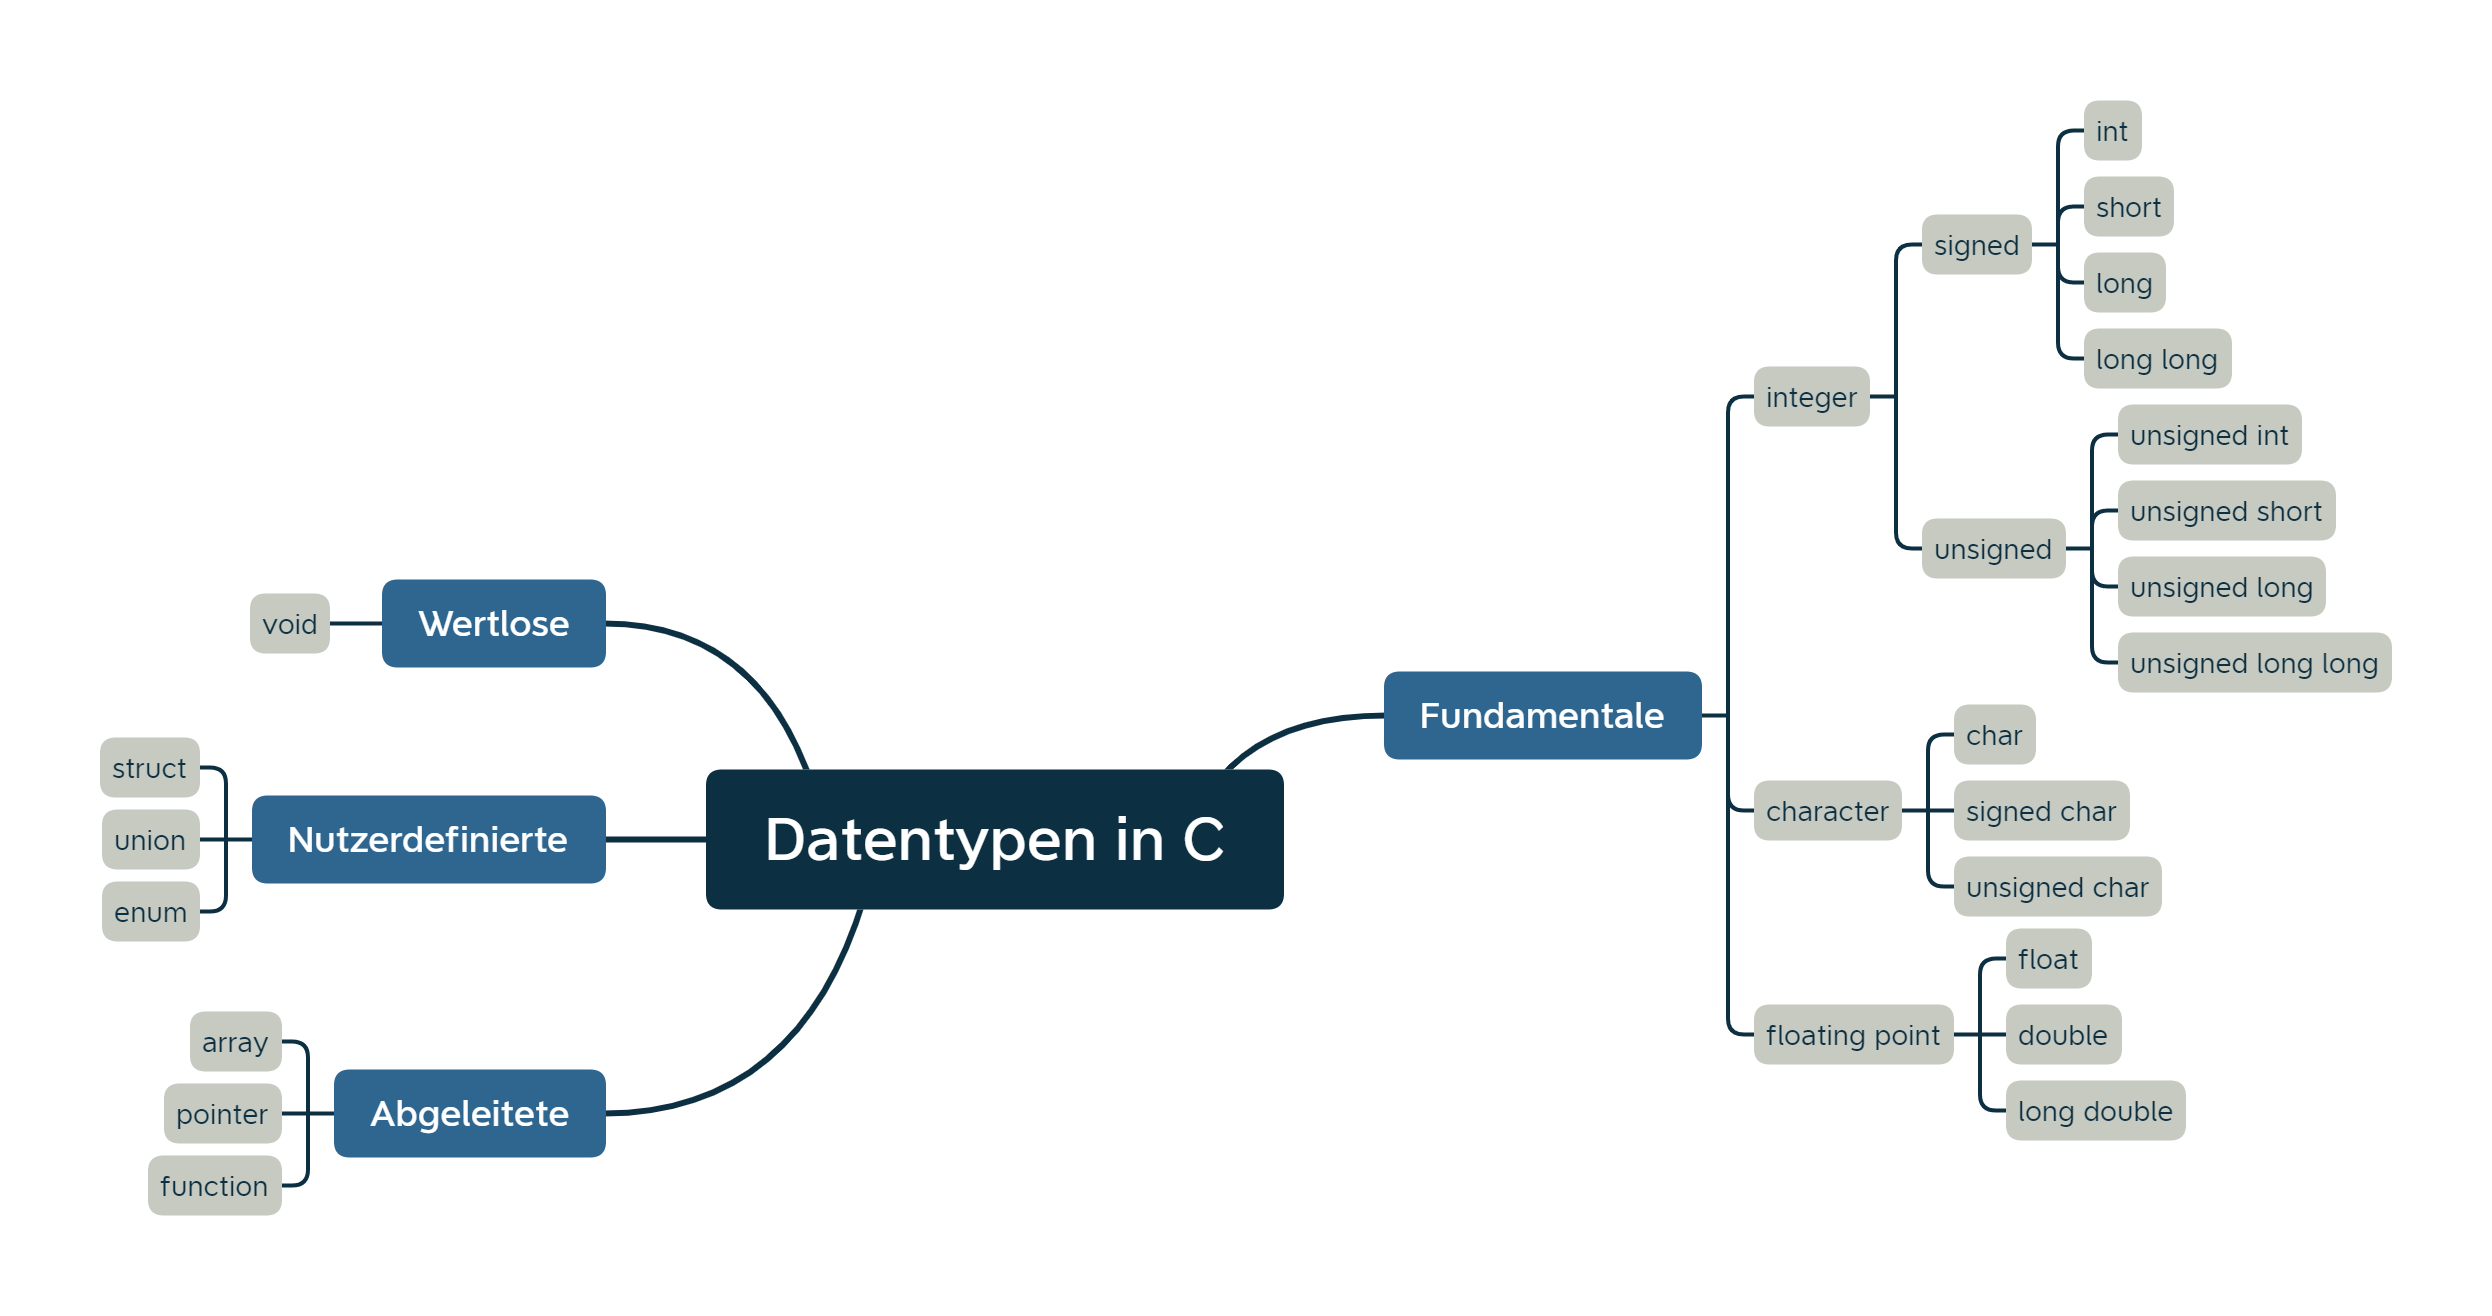
\includegraphics[width=\textwidth]{DatentypeninC.png}
    \caption{Datatypes in C}
    \label{fig:DatentypeninC}
\end{figure}

Understanding the significance of global and local scope in C is crucial for beginners as it fundamentally affects how memory is accessed, modified, and managed throughout a program. 
Global, declared outside of all functions, are accessible from any part of the program, making them useful for shared data or constants. 
However, their use can lead to code that is hard to debug and maintain, as any part of the program can change their values, potentially leading to unexpected behaviors.

Local identifiers, declared within functions, have a scope limited to their function, which enhances code modularity and reusability. 
They are created when the function is called and destroyed upon completion, reducing memory usage and preventing unintended side-effects outside their scope. 
This scoping helps in creating predictable and isolated behaviors for functions, simplifying debugging and understanding of the program.

Grasping these concepts is fundamental to writing maintainable and error-free code. 
It encourages good programming practices, such as minimizing the use of global variables, which can lead to more robust and secure programs. 
Moreover, understanding scope prepares new developers for more complex concepts like memory management, pointers, and concurrency, which are pivotal in C programming.

\section*{Exercises}
\begin{aufgabe}
    In order for us, to temporarily store values inside of our program, we need to understand how memory is allocated to a piece of data we'd like to store.
    Take a look at the following code snippet:
    \begin{lstlisting}[language=c]
        x = 0b0000111101011111;
    \end{lstlisting}
    The snippet shown is a so called \textbf{statement}.
    A statement is the fundamental unit of execution in a program.
    Statements are used to perform an action. 
    In the case shown, the action is to assign the value 0b0000111101011111 to the memory location indicated by the identifier \texttt{x}.
    Argue what the value of \texttt{x} can represent.
\end{aufgabe}

\begin{aufgabe}
    If your previous answer was: "I don't know", you're correct. 
    A bit-pattern as shown above, could potentially represent a whole variety of values, depending on the context and the use case.
    Right now, it is just a pattern, stored in memory.
    Even though it would be totally legal in \texttt{as} to for example \texttt{mov 0b0000111101011111 \%rdi}, in \texttt{C} this is not meant to be.
    We need to remember, that it is not us, writing the program, but the compiler.
    The abstract machine, which is responsible for the translation of the program into machine code, needs to understand, what we are trying to do here, and which operations are legal on any given piece of data.
    Thus, every identifier, that is declared in a C-program is bound to a particular kind of pattern of interpretation.
    These patterns are called \textbf{types} in \texttt{C}.
    Each time we declare a new identifier in C, we have to specify its type.
    Let us take a look at three fundamental types in C:
    \begin{enumerate}
        \item \texttt{int} - an identifier declared with this type is supposed to represent a whole number
        \item \texttt{char} - an identifier declared with this type is supposed to represent a single character
        \item \texttt{float} - an identifier declared with this type is supposed to represent a floating point number
    \end{enumerate}
    The declaration of an identifier in C looks like this:
    \begin{lstlisting}[language=c]
        int x;
        char y;
        float z;
    \end{lstlisting}
    After the declaration, the identifier is bound to its type and the compiler keeps track of it.
    It makes sure, that we are not declaring an identifier twice, or using an identifier that is not declared.
    Every new piece of data that we want to store in our program, has to be declared with an appropriate type.
    Look at the following two experiments and explain, why the return value changes:
    \begin{enumerate}
        \item \href{https://godbolt.org/z/nxK5z9fKf}{Example a}
        \item \href{https://godbolt.org/z/PG7GTPP4o}{Example b}
    \end{enumerate}
\end{aufgabe}

\begin{aufgabe}
    Without knowing to much yet about the \texttt{printf()} function, explain what you see:
    \begin{enumerate}
        \item \href{https://godbolt.org/z/f7M7bfaeK}{Example c}
    \end{enumerate}

\end{aufgabe}

\begin{aufgabe}
    The lifetime of an identifier is defined by the \texttt{\{}- and the \texttt{\}}-operators.
    A section in your code encapsulated by \texttt{\{} and \texttt{\}} is called a \textbf{scope} or \textbf{block}.
    Scopes can be nested in oneanother. 
    An identifier can only be used within its scope.
    Take a look at the following examples and explain what you see:
    \begin{enumerate}
        \item \href{https://godbolt.org/z/TErMKafjW}{Example d}
        \item \href{https://godbolt.org/z/GdbqM5b9h}{Example e}
        \item \href{https://godbolt.org/z/jhrsvsja6}{Example f}
    \end{enumerate}
\end{aufgabe}

\begin{aufgabe}
    Handling scopes and data-types correctly is one of the key parts in writing error-free code.
    It can also help you, keeping your RAM footprint under control.
    Take a look at the following examples and explain what you see:
    \begin{enumerate}
        \item \href{https://godbolt.org/z/eaG6f7q66}{Example g}
    \end{enumerate}
\end{aufgabe}

\section*{Annotations}
\begin{enumerate}
    \item The Compiler-Explorer - a beautiful tool for exploring C: \url{https://godbolt.org/}
\end{enumerate}

\end{document}
